\documentclass[border=2pt]{standalone}
\usepackage{pgfplots}
\pgfplotsset{compat=1.18}
\begin{document}
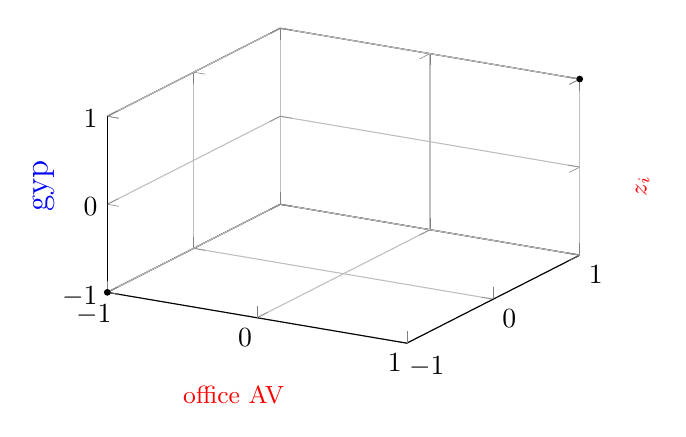
\begin{tikzpicture}
\begin{axis}[view={30}{30},scale only axis,width=6cm,height=4cm,
  xmin=-1,xmax=1,ymin=-1,ymax=1,zmin=-1,zmax=1,enlargelimits=false,
  xtick={-1,0,1},ytick={-1,0,1},ztick={-1,0,1},grid=major,
  xlabel={office AV},ylabel={gyp},zlabel={$z_i$},
  label style={font=\small,text=red,inner sep=2pt},
  xlabel style={at={(axis description cs:0.25,-0.1)},anchor=north,xshift=3pt,yshift=-2pt},
  ylabel style={at={(-0.1,0.5)},anchor=south,rotate=90,font=\large,text=blue},
  zlabel style={at={(axis description cs:1.1,0.5)},anchor=north,inner sep=3pt}]
  \addplot3[only marks,mark=*,mark size=1pt] coordinates {(-1,-1,-1) (1,1,1)};
\end{axis}
\end{tikzpicture}
\end{document}
